\documentclass[conference]{IEEEtran}
\IEEEoverridecommandlockouts
\usepackage{url} 
\usepackage{cite}
\usepackage{amsmath,amssymb,amsfonts}
\usepackage{algorithmic}
\usepackage{graphicx}
\usepackage{textcomp}
\usepackage{xcolor}
\def\BibTeX{{\rm B\kern-.05em{\sc i\kern-.025em b}\kern-.08em
    T\kern-.1667em\lower.7ex\hbox{E}\kern-.125emX}}

\begin{document}

\title{Power laws in code repositories: A skeptical approach\\
	\thanks{This paper has been supported in part by
		project DeepBio (TIN2017-85727-C4-2-P)}
}

\author{\IEEEauthorblockN{1\textsuperscript{st} Bartolom\'{e} Ortiz}
	\IEEEauthorblockA{\textit{Geneura Team,ETSIIT and CITIC} \\
		\textit{University of Granada}\\
		Granada, Spain \\
		bortiz@ugr.es}
	\and
	\IEEEauthorblockN{2\textsuperscript{nd} J. J. Merelo}
	\IEEEauthorblockA{\textit{Geneura Team,ETSIIT and CITIC} \\
		\textit{University of Granada}\\
		Granada, Spain \\
		jjmerelo@ugr.es}
}

\maketitle

\begin{abstract}
  
Software development as done using modern methodologies and source
control systems has been often established as an example of
self-organization, with code growing and evolving organically, through
activities that do not stem from centralized power, leader or
directives.  The main challenge is proving these claims is that self
organization cannot be detected through direct observation, but
through measurements on the system, looking for hints such as the
existence of powerlaws over some features, such as the size of changes
over time.  The problem we intend to tackle in this paper is to check,
for a chosen set of repositories we had already measured in the past,
if the claims about power laws actually holds from a precise
mathematical point of view, since, although shown as pervasive in the
software engineering literature (and others), power laws are more
elusive than they might seem at first sight. For that reason, in this
paper we present a statistically accurate set of tests that will help
us decide, from the way repositories are changing, if they are really
distributed by a power law, which could indicate us the existence of a
state reached via self-organization, or actually, how accurately a
power law fits the observed distribution of the size of changes of
commits in git repositories of 16 open source repositories.  We
revisit one of the most representative papers of these observations to
reevaluate its results and compare them with the current status of the
repositories analyzed in it, trying to elucidate if there has been any
change in the possible presence, or not, of a power law.

\end{abstract}

\begin{IEEEkeywords}
	Complex systems, self-organizing systems, self-organized criticality, power laws, software development, 
	software repositories
\end{IEEEkeywords}


%%%%%%%%%%%%%%%%%%%%%%%%%%%%%%%   INTRODUCTION   %%%%%%%%%%%%%%%%%%%%%%%%%%%%%%%
\section{Introduction}\label{introduction}

There are several steps in the study of self-organized systems  \cite{bak1988self}. One of
them is to study the existence of a power-law's distribution in the data
from our system. This property is intrinsically related to the scale-free behaviour
these systems exhibit, that is, systems where there is no single characteristic event size \cite{golyk20self}.
Understanding what distribution is producing our data gives us insights of
how confidently we are about claiming that our system is in a critical state, since this states
are usually correlated with the appearance of a power law \cite{newman2005power}. % cite needed -bart

Moreover, it is interesting to see if there is some kind of evolution in the distribution the data follows. 
A change in the distribution that explain the data could be originated by a 
phase change, and a phase change happens by getting to a critical state. % I don't like how this sentence is built... Too roundabout - JJ

However, during the process of investigating the existence of self organization, or the change to a critical state, we have to justify every conclusion we get, not only 
by fitting our data, but by giving a proper statistical measure of the probability 
of our conclusions, that is, following an standardize mathematical method based on
hypothesis testing.

% * Why is self-organization in repositories important? What would it imply -JJ
% I 'm not sure about how to "attack" this question. - Bart
In our case, we are mainly interested in code repositories. The
existence or not of a critical state is essential to understand the
processes taking place in free software repositories, which are
sometimes partly or fully based on volunteer work. In these cases,
sustainability is the main objective, and understanding how
self-organization relates to productivity and to the continuous
collaboration of volunteers is essential to keep a software team
healthy. Also, understanding the micro-mechanisms through which
self-organization takes place provides insights on the possible
incentives to avoid churn of volunteers, as well as to make their work
add as much value as possible to the project.

Following \cite{merelo16:self,Merelo2016:repomining,merelo17vue,DBLP:conf/iwann/MereloCV17,merelo2017self} approach, we are going to try and comprehend code repositories
by the interactions (events) made in them. Code repositories are one
of the main ways 
software is developed nowadays. Multiple platforms like GitLab or GitHub 
offer the possibility of interact with the code making changes, adding and deleting 
lines. 
All these interactions are reflected in an archive by the so called
commits. From this archive
we can obtain the data about how this code has been changed. Although
these changes sometimes obey issues with the code, or bug fixes, in
many cases they simply are piecewise improvements or code changes that
are decided by programmers themselves. 

But to really start to understand the behavior and possible self-organization of software development teams as
reflected by their activity in repositories, we should not
only try to fit a power law in our data but try to make a statistically
accurate study to confirm how much evidence we have of this type of
behavior. 

Most of the measures and estimations about power laws in code repositories are collected 
in studies like \cite{merelo2017self}, where some evidences of power laws are presented.
However, since there are better methods to study this data \cite{clauset2009power}, 
we are going to re-evaluate all the results obtained, offering an alternative skeptic view
of the existence of power laws, following recent papers such as \cite{Holme2019,Broido2019}.

We have focused in this particular topic because of three reasons.\begin{itemize} 
\item First of all, there are no 
extensive analysis that addresses this question. We haven't found a comparative study 
that offers data-based statistical measures to check if the power law assumptions hold.
So we are going to fill this gap offering a complete statistically study about
the evidences of power laws behavior in a variety of repositories.
\item Moreover, we are not going to evaluate just our evidences about the existence of a power law,
we are going to offer a short range of distributions that can generate similar results and could
easily be confounded by a power law. This is an standard way to discover if our data is more likely
to be produced by other heavy-tailed distribution \cite{clauset2009power}, like the logNormal
or the truncated power law. 
\item 
Finally, since we are able to access to multiple years' data, we also interested in study the
temporal evolution of the two previous analysis. Here our main objective is to show how these measure could 
have changed (if they have at all). We should remember that repositories are evolving system
by definition, so they can experiment qualitative changes in his events distribution. Furthermore, even 
if they preserve their behaviour, they can still change some distribution's parameters.
To locate and analyze this changes could be translated in a deeper knowledge in the evolution 
of these system, specially in the presence of phase changes \cite{merelo2017self} or self-organized
critically (understood as a mechanism by which the system is regulating himself to stay in those 
parameters \cite{newman2005power}).
\end{itemize}

This way, we offer a test to analyze how much evidence there is for or
against our assumptions in every step, and a set of comparatives to
identify some relevant temporal 
changes, establishing a statistically correct starting point to answer
the question: Does software 
development really follows a power law? 

Next, we will explain our methodology followed by the results obtained,
closing with our conclusions. 

% --------------------------------------------------------


\section{State of the art}\label{soa}

The study of code repositories from the point of view of self-organized criticality has not followed a continuous line of investigation.

On the one hand, we find that self-organized criticality has been
Description of a wide variety of code repositories with a certain probability. These studies can be found in\cite{wu2007empirical,gorshenev2004punctuated}, but they are not the only ones of this kind. Tests on the possible self-organized criticality have also been sought in another type of repositories and projects, which are enumerable in size and purpose \cite{Merelo2016:repomining,merelo16:slash,merelo16:self,merelo2017self}.

In most of these studies, however, the evidences in favor of the existence of a power law are not accompanied by a significant statistical study. It is usual, as described in \cite{newman2005power} that the evidence leading to a suggestion of a power law in the distribution is visual. Once we have these tests, the study goes through the adjustment of a possible powerlaw \cite{merelo2017self,arafat2009commit}.

The general trend being the lack of statistical evidence that supports the hypothesis of the existence of a power law, the truth is that as described in \cite{newman2005power, clauset2009power} the most common method for making subsequent adjustments, Leas Square Medium \cite{merelo2017self,arafat2009commit,merelo16:self}, usually implies the existence of a greater error than the possible alternatives.

Currently, the general trend that started with the description of the power laws in self-organized systems has been slowed down. Instead, due to the existence of more objective evaluation methods, the results that were assumed until now are being re-evaluated.

Examples of this trend are papers such as \cite{Holme2019, Broido2019}, where the power laws in the networks and in the results have been reevaluated, obtaining an analysis that can change the way we make our assumptions about power laws.


Next we will present the methodology used to choose those repositories and
mine their information. 


% --------------------------------------------------------


\section{Methodology}
\label{sec:method}

\subsection{Data extraction}
We have chosen 16 repositories in different states of development.
These repositories were chosen in \cite{Merelo2016:repomining}, for several reasons:  They all represent a wide array of languages and functionalities, from web frameworks such as Django to Atom plugins, through one-of-a-kind frameworks such as Docker.

 Normally a code repository is related to a software project, for this reason, it is usual that they include several
different languages which are used in different parts of the project.
This mixture of languages also offer a big range of variability between languages that are interpreted or compiled, either to machine code or to
bytecode. 

Repositories vary also in {\em professionalism}, that is, the team behind that software project. From a small Atom editor plugin to TensorFlow, an open library created and maintained by a fully professional community.

Repository mining was done during the months of January to March
2017, with the second sweep of the same repositories performed in
February 2019.

The way we look at changes in the repository was initially proposed by \cite{Merelo2016:repomining} and was also used in
\cite{merelo2017self}, where a deeper explanation can be found.

% We need to rewrite all of this.
This procedure is based on three main concepts:
\begin{itemize}
	\item The usage of a discrete timeline formed by the
	commits, with every commit counting as time=1. 
	\item Work with selected files in the repository, excluding 
	those related to images or style
	\item We take the largest value from the inserted and deleted lines of code.
\end{itemize}

Up to this point, there is nothing new. But is the way that we evaluate our results that differs from previous analysis.

\subsection{Hypothesis tests}

Once the information from the repositories has been extracted, we
proceed to analyze it in order to find clues about what kind of distribution is generating our data. 

With that particular objective in mind, we change the methodology used
in \cite{merelo2017self} for several reasons.

First of all we want to offer a test that checks whether the observed data 
set actually follows a power-law, instead of only visualize the result. 
This kind of tests can vary based on different measured and techniques. The one we
are going to use is suggested in \cite{clauset2009power}, which consists in using a
goodness-of-fit hypothesis test via bootstrapping procedure. 

Due to the use of bootstrapping, this procedure is a time and resources consuming one.
We essentially  generate  multiple  data  sets  with our two main parameters $x_{min}$ 
and $\alpha$  and  then  we re-infer the model parameters. The outcome of the algorithm 
will result in a P-value, which, if is large enough, tell us that the difference
between our data and the power law model we have generated is small and mostly attributed
to statistically randomness. On the other hand, if P-value is close to 0, it is quite unlikely
that our model fits the data properly.
Following \cite{clauset2009power} we choose our threshold value in $p=0.01$, in addition
we are going to perform this analysis with R package: PoweRlaw. A detailed description
of it and the hypothesis tests can be found in \cite{gillespie2015power}.

Up to this point, we have detected what data sets are unlikely to be fitted by a power law
in any of its range. Notice, on the contrary case, that we are only assuming that
we can not discard that a power law is generating the data.
However, as there is some probability of the appearance of this distribution in our data
we can study and analyze how its two main parameters may evolve between 2017 and 2019.

As it is unrealistic to think that a power law distribution will
fit all our data, our first step is to check what portion of the data
could be fitted with a power law, or in other words, what is the minimal value 
(if there is one) from which the scaling relationship of the power law begins
\footnote{This is a fair assumption since we are working with heavy-tailed distributions 
	and our main interest is the behaviour of the tail of our data.}. 
This value is usually noted by $x_{min}$ and is our first parameter.

Once we have the first value, we proceed to estimate the scale of our power law.
As it is shown in papers like \cite{newman2005power, clauset2009power},
least square method is a poor but wide-spreaded way to proceed when estimating the
scale parameter. Instead, we are going to use a direct method describe in
\cite{clauset2009power} and implemented in \cite{alstott2014powerlaw} that use
the data values we have. This method is known to produce a very nice fit with
less error than the others mentioned above.

Up to this point we have revisited our way of analyze power law fitting and
the estimation of our parameters. However, there is a more deep question unanswered:
does our data really follow (in a statistically relevant way) a power law?
This kind of answers were lacking in \cite{merelo2017self} and they are relevant
independently our first test's results, since they usually offer an unbiased look of the data . 

Taking into account that our main question is wether a power law is the best 
description of our data, we choose to apply a comparative test that could 
evaluate if there are any alternative distribution that could have generated
our data with greater likelihood than a power law. That is the main reason why
we choose to use a log-likelihood ratio test implemented in \cite{alstott2014powerlaw}.
There are two algorithm's outcomes. First we have the log-likelihood ratio between the 
two  candidate  distributions. The sign of this quantity will point out which
distribution is more likely to be producing out data. After it, we calculate the signification 
of this ratio, a P-value. Following \cite{alstott2014powerlaw} indications we establish our P-value threshold at $p=0.05$;
above that point the loglikehood ratio has no significance and we can not decide which distribution
is better fitting out data.

\subsection{Classification}

With all this information we are able to offer a precise conclusion about the 
probability that power law is generating our data. To sum up all the tests in a single 
statement we use the scale proposed in \cite{clauset2009power}, which is described as:
\begin{itemize}
	\item \textbf{None}: Data-set is probably not distributed by a power law (first test failed).   
	\item \textbf{Moderate}: Power law is a possible fit but there are other plausible distributions that fit the data.
	\item \textbf{Good}: Power law is a possible fit and none of the other distributions is plausible.
	\item \textbf{Truncated}: when truncated power law is clearly favored over a simple power law
\end{itemize}


\subsection{Visualization}
 
On the visual aspects, an aclaration should be made. Here we offer a graphical view that differs from \cite{merelo2017self}
but not a novel one. It has been used in \cite{arafat2009commit} with similar purposes. 
Briefly, we are going to use the probability density function (PDF) for plotting. Due to the 
requirement of binning the data to this type of graphic, we are going to use a
logarithmic spacing, since it reduces the statistical errors in the tail in log-log 
plots at it is stated in \cite{newman2005power}.


% --------------------------------------------------------


\section{Results}
\label{res}
% % Is this really needed?
First, analyzing the parameters of the possible power law distribution, we find that in those repositories with low variation of the $x_{min}$ parameter there is a lack of correlation between the changes in the estimated starting point from which the distribution of power law starts and the scale parameter, $\alpha$. Even if small changes in $xmin$ produce small changes in $\alpha$, the lack of correlation probably means that this changes 
are the result of the natural stochasticity of the evolution process.  % What is the implication of this? This is a conference, it's not a Maths conference, you need to really explain what this is about- JJ

However, as can be seen in tables \ref{tab:2017pars} and \ref{tab:2019pars}, repositories such as Django, which have a strong variation in the initial point, also have a greater variation in the scale parameter. This is produce because of a change in the overall distribution. The structure of power law is starting in other point of the data which obviously results in a different power law fit that is probably different from the 2017's fit  % Implying what? - JJ


Another special remark should be addressed to Tensorflow. The distribution fit of the repository 2019 has been a little controversy between \cite{alstott2014powerlaw} and \cite{gillespie2015power}. We believe the main reason for that is the two different section detected by their algorithms. However, in both cases results produce similar results in the tests.


After analyzing the parameters analysis the results of the hypothesis test can be found in Tables \ref{tab:2017tests} and \ref{tab:2019tests}. 

We can observe that in general, as the repositories evolve over time, there is a tendency to the appearance of a greater probability in favor of power law existence, as None cases have been reduced between 2017 and 2019.

Even so, it is worth noting the complete lack of repositories in which our confidence in finding a power law distribution is high (following our scale: \textit{Good}).

Faced with the most common visualizations, the one used in our paper highlights even more how we can not affirm the existence of power laws distributions if we look at them in detail. See as an example how Fig. \ref{fig:docker}. shows that the adjustment of a power law would not capture some characteristics in the tail of our data. 

We would like to remark that, even in smaller plots like \ref{fig:pl2017} and \ref{fig:pl2019}, where we could easily say that there are power laws only by sight, the mathematics presented in this paper support that the probability of that happening is, as maximum, \textit{ moderate}.

A proper example of this kind of biased assumptions is Fig. \ref{fig:mojo}. Seen the Mojo distribution and power law fit we can suspect the existence of a power law in the repository. Its distribution that also remains in time till 2019. This can be an indicative that this repository is self-organizing to stay in that point. But even in this case, the probability of a power law is only, again, \textit{moderate}.

% The whole idea about using .Rnw is to have this generated automatically. Maybe next time - JJ
\begin{table*}[htbp]
	\caption{2017 Parameters with power law fitting}
	\begin{center}
		\begin{tabular}{| p{0.12\linewidth} | p{0.1\linewidth} | p{0.3\linewidth} | p{0.3\linewidth} |}
			\hline
Repository name &$x_{min}$ & $\alpha$ & $\sigma$\\
\hline
atom &10.0 &2.039242998376567  &0.15492119930071382 \\
cask &18.0 &1.7336857967225443  &0.06725686671465021 \\
Dancer2 &107.0 &2.177500075690754  &0.07730666731550309 \\
django &10786.0 &2.1744317304939558  &0.01917838984962695 \\
docker &73.0 &1.4645926562553306  &0.004754872537365103\\
ejabberd &2.0 &1.228631569923214  &0.0033017325614456455 \\
fission &25.0 &1.7697310637483803  &0.09937185303186655 \\
mojo &32.0 &2.1283668081735456  &0.03162540535355575 \\
Moose &36.0 &1.768059278495766  &0.0197132783524576 \\
rakudo &11.0 &1.6159534004325067  &0.006834230629556248 \\
scalatra &105.0 &1.7126278313239238  &0.02583273870367301 \\
tensorflow &6.0 &1.2136744934008  &0.002587381661200525 \\
tpot &39.0 &1.601798428793051 &0.0374663336679551 \\
tty &85.0 &2.5687968664786887  &0.16355837969418938 \\
vue &10.0 &1.4008340778667951  &0.007381204719143647\\
webpack &66.0 &1.7525127838915868 &0.030568742256899546\\ 
			\hline
		\end{tabular}
	\end{center}
\label{tab:2017pars}
\end{table*}


\begin{table*}[htbp]
	\caption{2019 Parameters with power law fitting}
	\begin{center}
		\begin{tabular}{| p{0.12\linewidth} | p{0.1\linewidth} | p{0.3\linewidth} | p{0.3\linewidth} |}
	\hline
	Repository name &$x_{min}$ & $\alpha$ & $\sigma$\\
	\hline
atom  &9.0  &1.8359195263285408  &0.11705214645679832 \\
cask  &22.0   &1.7974451838770937  &0.07249501671609943 \\
Dancer2  &106.0   &2.261037545006354  &0.08425661509414822 \\
django  &22380.0   &2.6887068697480156  &0.03580856180986959\\
docker  &85.0  &1.471139237773135  &0.004450258248742491 \\
ejabberd  &4.0   &1.2671552485187476  &0.00372055095134032 \\
fission  &22.0   &1.4589753590316525  &0.021399836458042016\\ 
mojo  &32.0   &2.1384964656994434  &0.031043490328162827 \\
Moose  &36.0   &1.7677961781806713  &0.019622681314368864 \\
rakudo  &12.0   &1.603181925304308  &0.006028504486885445 \\
scalatra  &105.0  &1.678355887867916  &0.02363164712583398 \\
tensorflow  &16.0  & 1.276851335699674  & 0.0017743964236792348 \\
tpot  &176.0   &2.139617006349855  &0.08401368034180524 \\
tty  &83.0   &2.6669971731409587  &0.1582243695783554 \\
vue  &12.0   &1.4407170088980175  &0.007474075257736019 \\
webpack &50.0  &1.481958114820392  &0.00906295021690492 \\
			\hline
		\end{tabular}
	\end{center}
\label{tab:2019pars}
\end{table*}


\begin{table*}[htbp]
	\caption{2017 summary results}
\begin{center}
	\begin{tabular}{| c |c| c | c| c |c | c |}
		\hline
		Repository name & KS test & PL vs. LogN & PL vs. Exp & PL vs. PLtrunc & Result \\ 
		\hline
		atom & 0.244 &ND & ND &PLtrunc & Truncated \\ 
		cask & 0.236 &ND & PL & ND & Moderated \\
		Dancer2 &0.178 &ND &PL &ND & Moderated \\
		django &0.002 &LogN &PL &PLtrunc &None\\
		docker &0 &LogN &PL &PLtrunc &None\\
		ejabberd &0 &LogN &PL &PLtrunc &None\\
		fission &0.654 &ND &PL &PLtrunc &PLtrunc\\
		mojo &0.874 &PL &PL &ND & Moderated \\
		Moose &0.2 &PL &PL &PLtrunc & PLtrunc\\
		rakudo &0 &PL &PL &PLtrunc & None\\
		scalatra &0 &LogN &PL &PLtrunc & None\\
		tensorflow &0 &LogN &PL &PLtrunc & None\\
		tpot &0.01 &LogN &PL &PLtrunc &None\\
		tty &0.418 &ND &ND &ND & Moderated \\
		vue &0 &PL &PL &PLtrunc & None\\
		webpack &0.004 &LogN &PL & PLtrunc & None\\
		\hline
	\end{tabular}
\end{center}
\label{tab:2017tests}
\end{table*}

% Can we maybe show all repos in the past and now? Would that be useful? - JJ

\begin{table*}[htbp]
	\caption{2019 summary results}
	\begin{center}
		\begin{tabular}{| p{0.12\linewidth} | p{0.08\linewidth} | p{0.08\linewidth} | p{0.08\linewidth} | p{0.1\linewidth} |p{0.13\linewidth} | p{0.09\linewidth} |}
			\hline
			Repository name & KS test & PL vs. LogN & PL vs. Exp & PL vs. PLtrunc & Result \\ 
			\hline
			atom &0.108 &ND &ND &PLtrunc & Truncated \\
			cask &0.276 &ND &PL &ND & Moderate \\
			Dancer2 &0.426 &ND &PL &ND & Moderate \\
			django &0.862 &LogN &PL &PLtrunc &Truncated \\
			docker &0.118 &LogN &PL &PLtrunc & Moderate \\
			ejabberd &0 &LogN &PL &PLtrunc & None\\
			fission &0 &ND &PL &PLtrunc & None \\
			mojo &0.88 &PL &PL &ND &Moderate \\
			Moose &0.224 &PL &PL &PLtrunc &Truncated \\
			rakudo &0 &PL &PL &PLtrunc & None \\
			scalatra &0 &LogN &PL &PLtrunc & None \\
			tensorflow &0.418 &LogN &PL &PLtrunc & Moderate \\
			tpot &0.184 &LogN &PL &PLtrunc & Truncated \\
			tty &0.47 &ND &ND &ND & Moderate \\
			vue &0 &PL &PL &PLtrunc & None \\
			webpack &0.002 &LogN &PL &PLtrunc & None\\
			\hline
		\end{tabular}
	\end{center}
\label{tab:2019tests}
\end{table*}

% following pictures take too long to compile everytime we create the pdf, so I
% create them out of the document.
\begin{figure*}[htbp]
	\centerline{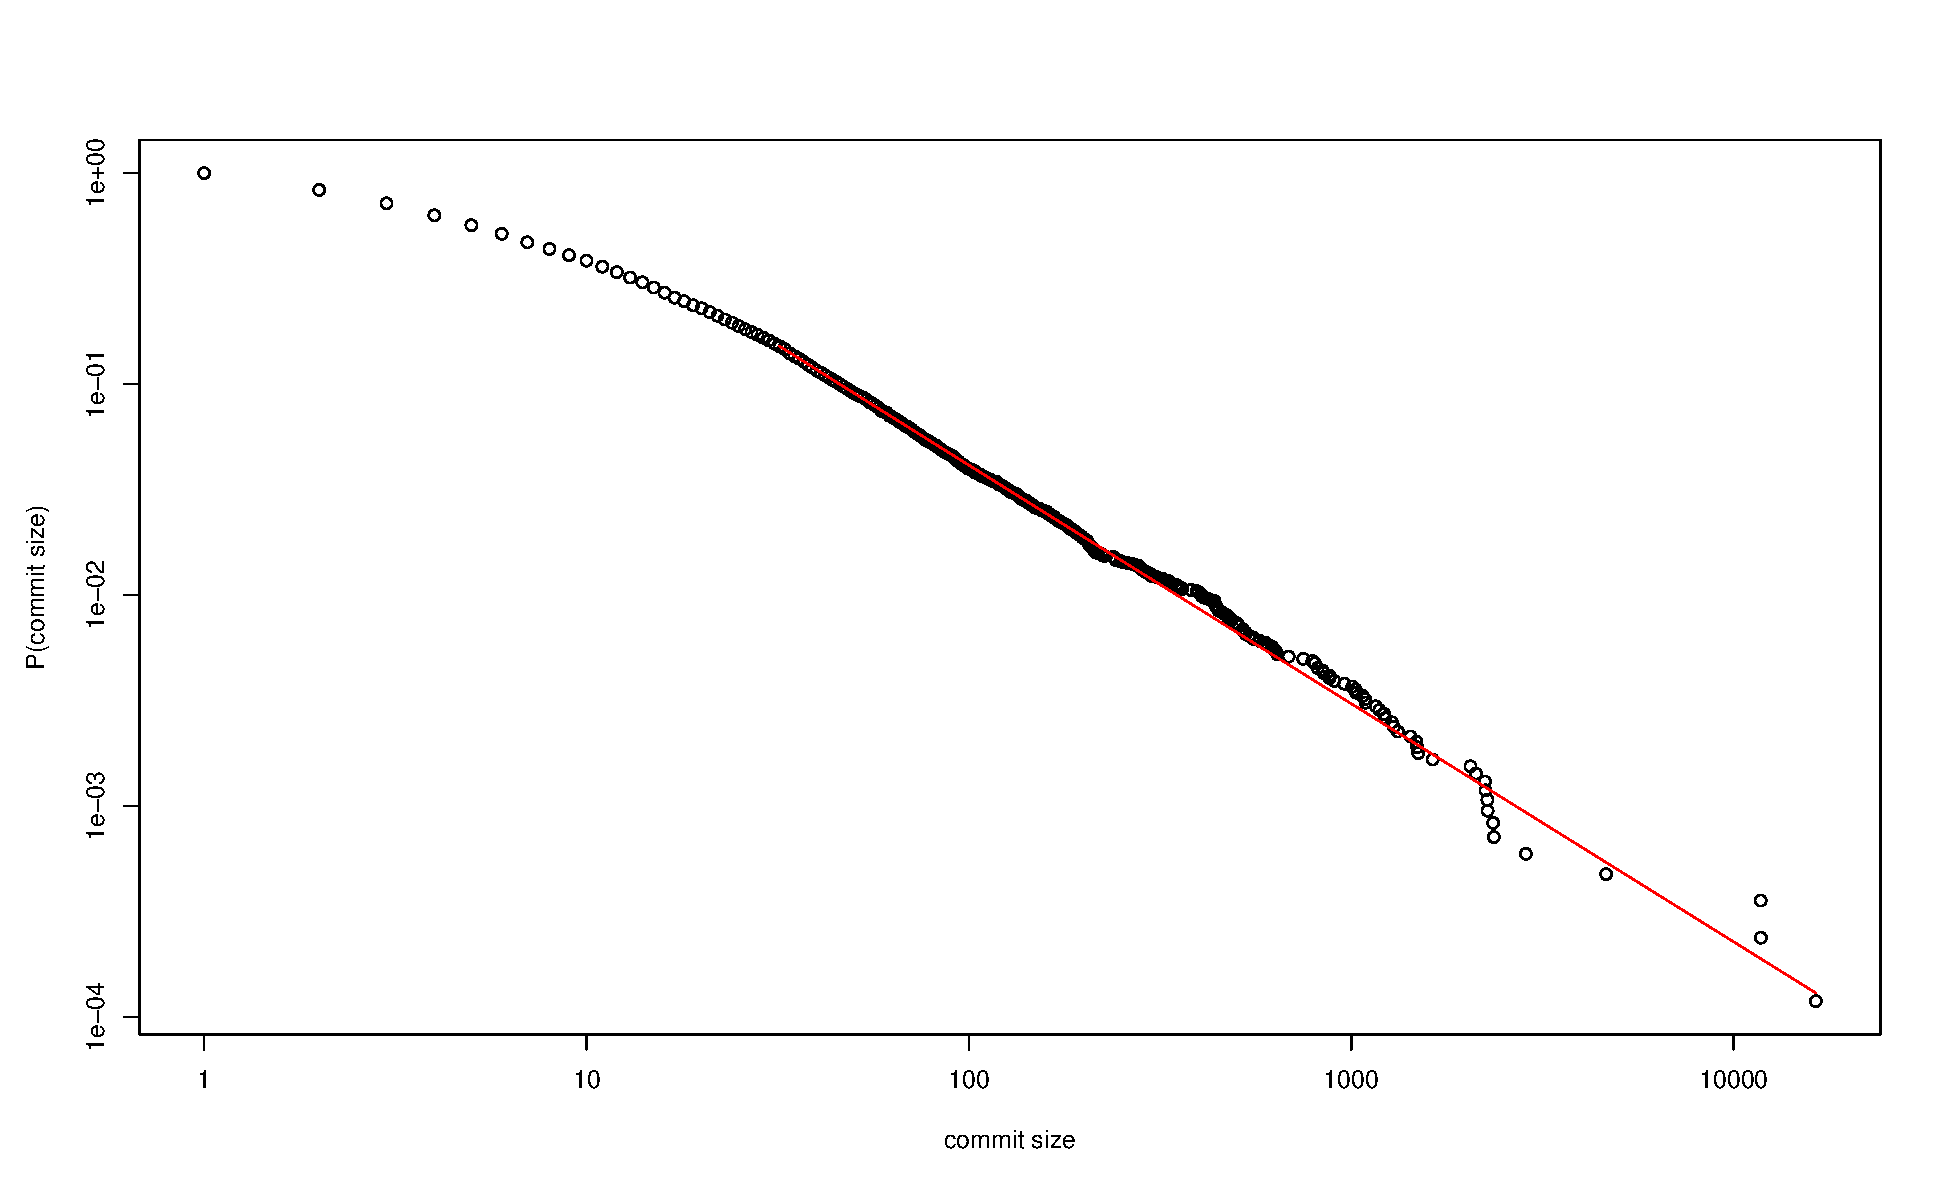
\includegraphics[width=0.95\textwidth]{plots/mojo-2017.eps}}
	\caption{PDF plot of a repository with \textit{Moderate} rank: Mojo from 2017.}
	\label{fig:mojo}
\end{figure*}



\begin{figure*}[htbp]
	\centerline{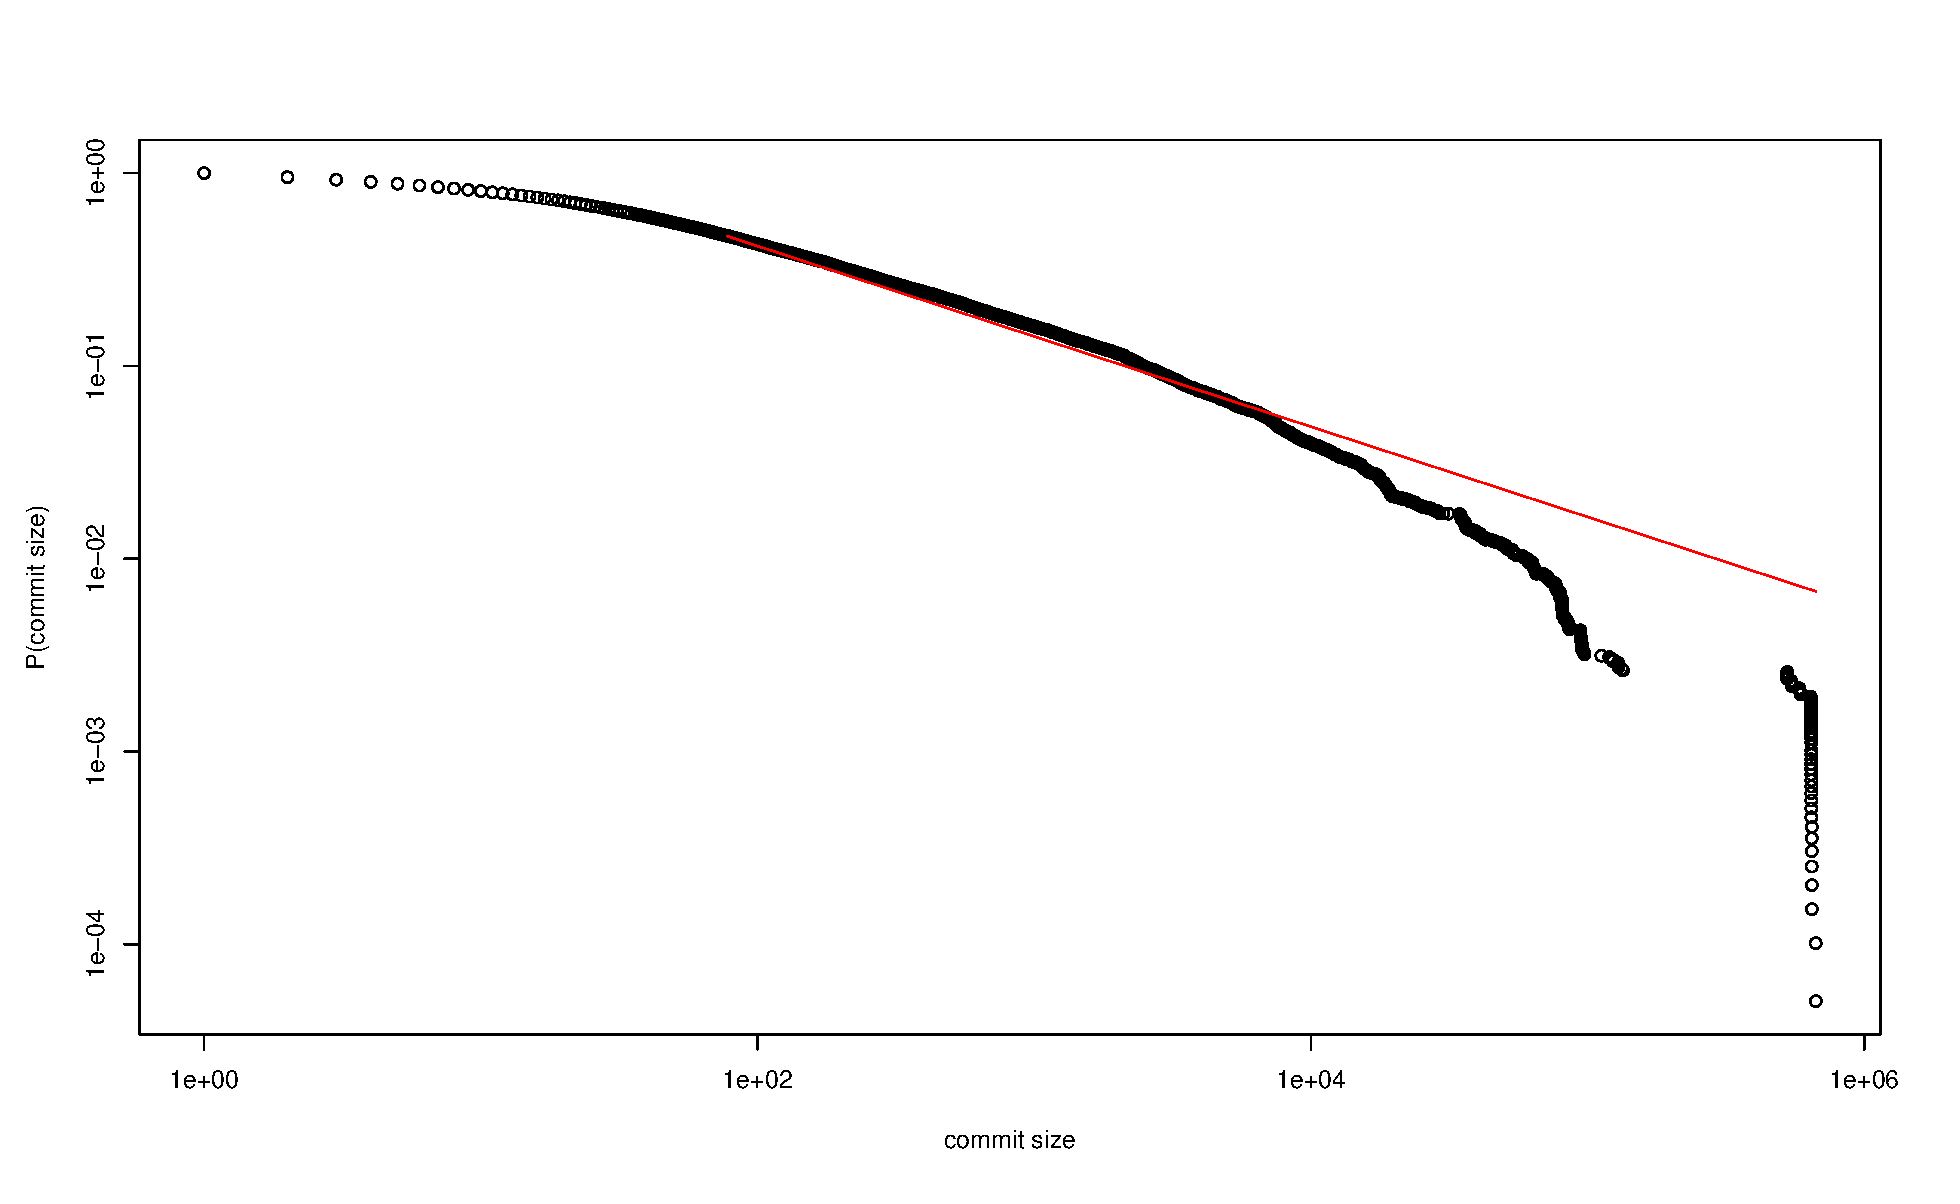
\includegraphics[width=0.95\textwidth]{plots/docker.eps}}
	\caption{PDF plot of a repository with \textit{None} rank: Docker from 2017.}
	\label{fig:docker}
\end{figure*}



\begin{figure*}[htbp]
	\centerline{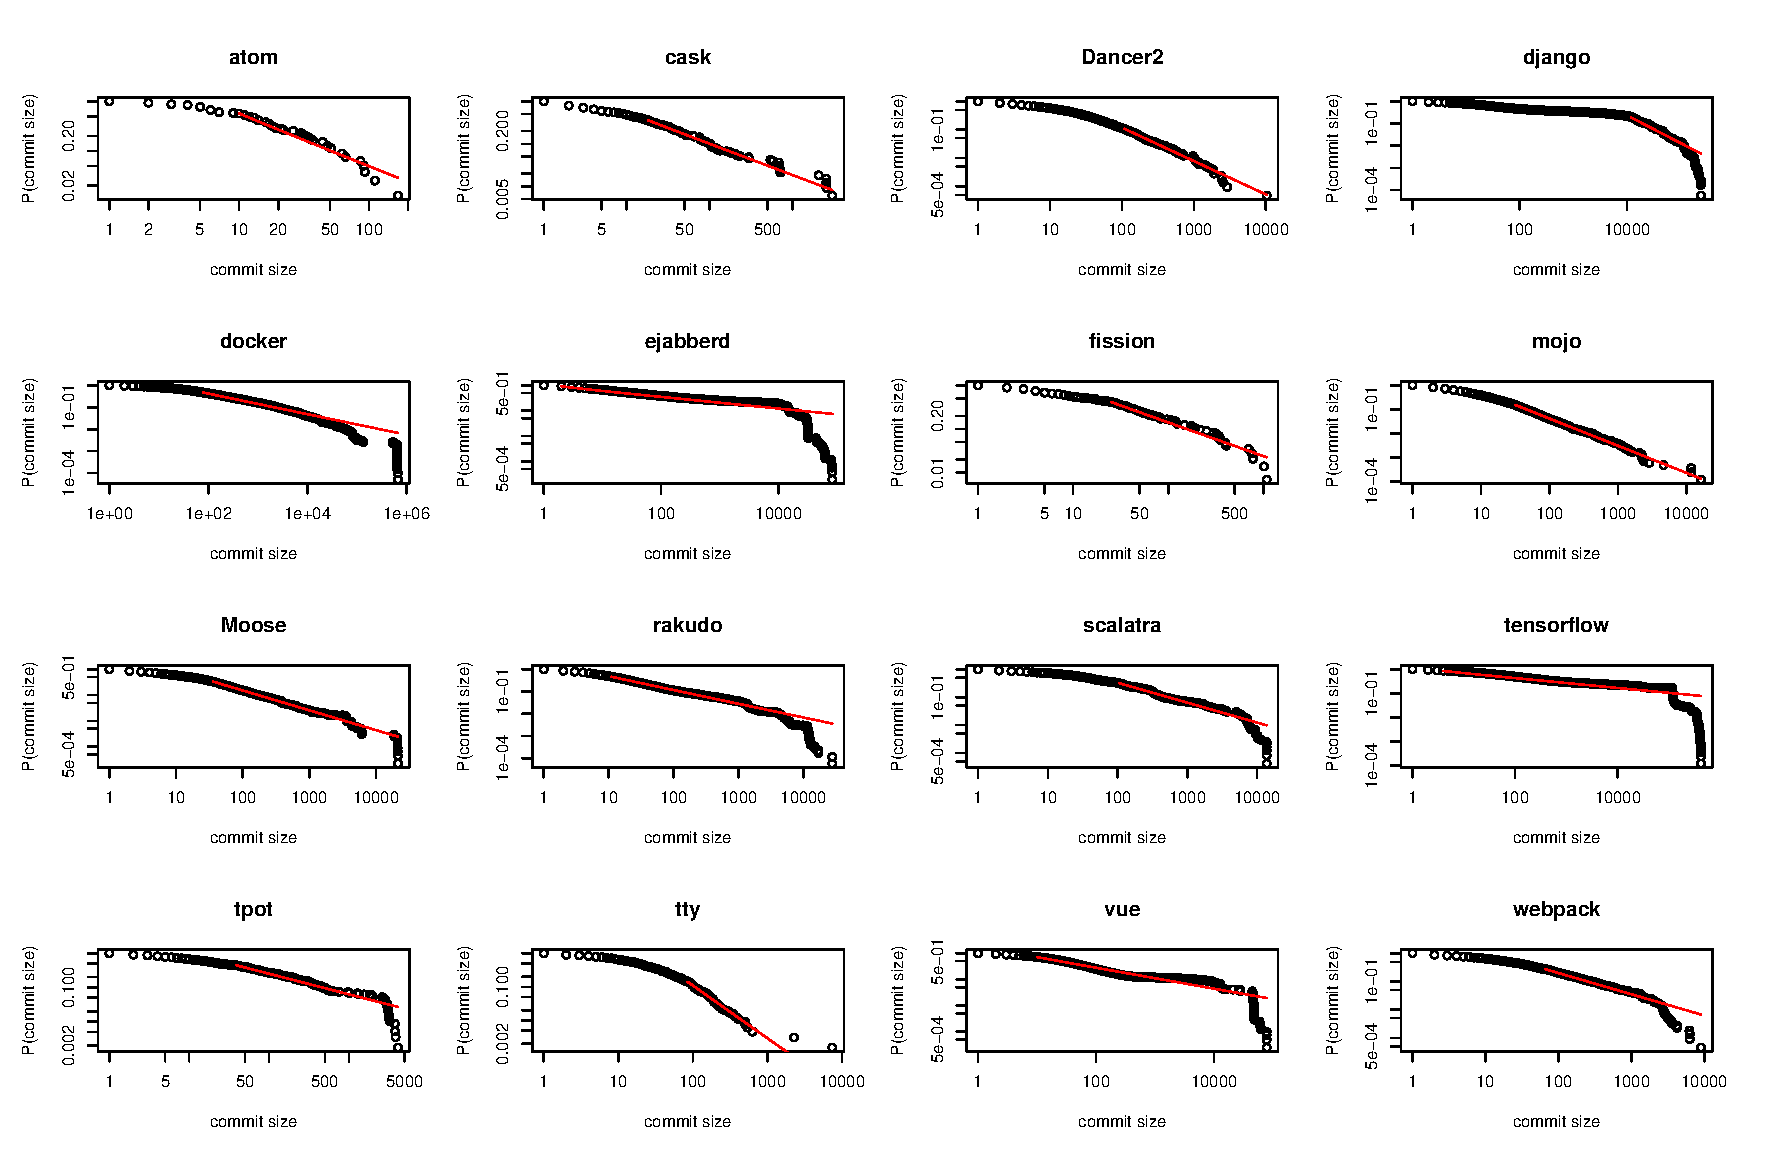
\includegraphics[width=1\textwidth]{plots/pl2017.eps}}
	\caption{PDF plot of all repositories 2017. Red line represents the power law fit}
	\label{fig:pl2017}
\end{figure*}



\begin{figure*}[htbp]
	\centerline{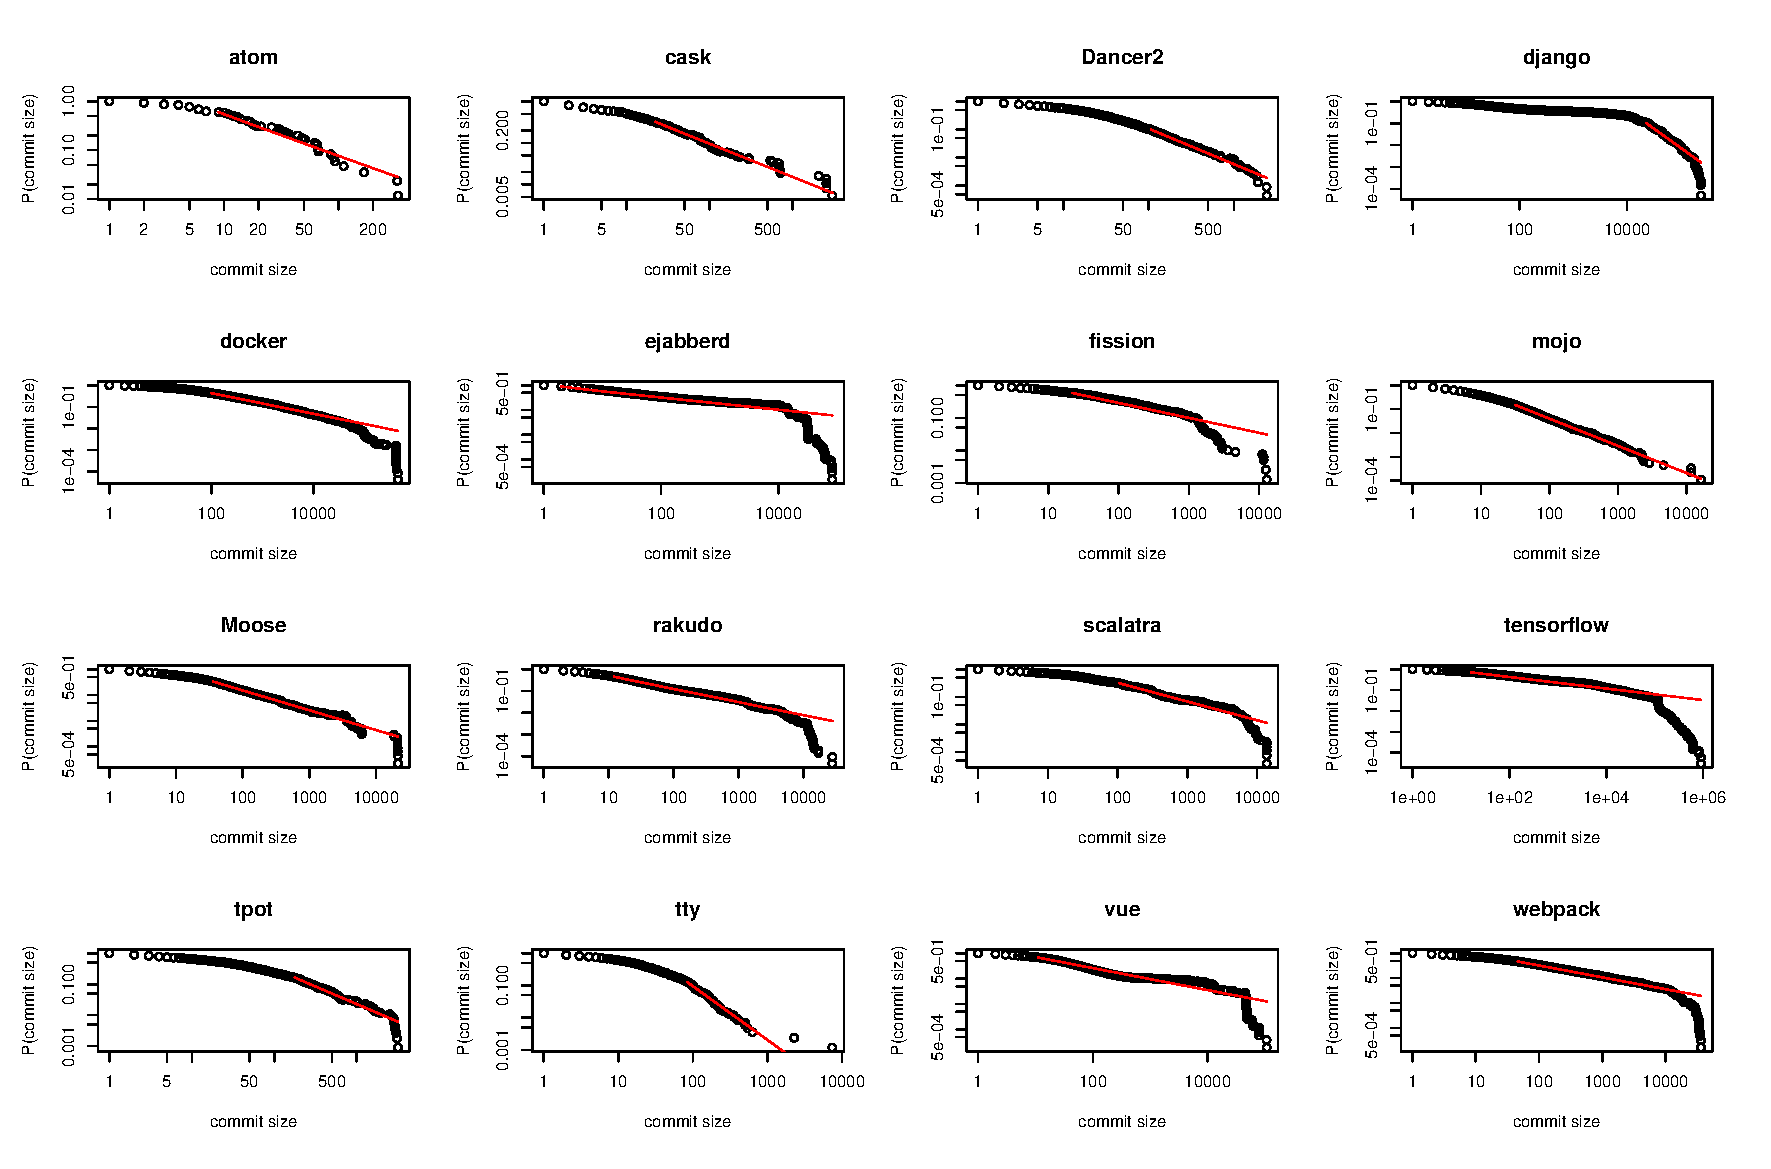
\includegraphics[width=1\textwidth]{plots/pl2019.eps}}
	\caption{PDF plot of all repositories 2019. Red line represents the power law fit}
	\label{fig:pl2019}
\end{figure*}

% --------------------------------------------------------


\section{Conclusions}\label{conc}


% Several things we can do in the conclusions
% * So, most repositories are _not_ actually self-organized because they do not follow a power law? Answer: We can't affirm that. Power laws only manifest themselves in critical states; self-organization will still take place. 

In conclusion, we should always use a standard mathematical approach in order to affirm any behaviour in our data's distribution. That way, we can assure that our results are unbiased (not based in our sight or plots) and they have been tested statistically. %That's not a very good conclusion... That should be the conclusion to the conclusion - JJ

In general, the probability of finding a power law  in the repositories studied is quite low, so, up to now, we can not affirm categorically that the system is in a critical state due to self-organization.

This result, however, does not imply that there is not any kind of self-organization or even a power law, but that the system has not been regulated enough and, therefore has not been established near a possible critical state.

% Figures should be referenced in the results section, not the conclusions. - JJ


Furthermore we would like to explore the possible causes of such dramatic changes as the ones seen in repositories like Django, since they can be related to a possible phase change.

In any case, the article presents an adequate and objective workflow to study the existence of power law distributions that settles the status of these kind of measures in software development via repositories.

Thanks to this procedure, we hope we can constitute a new state of art, from which researchers can begin to study these and other properties of code repositories in order to understand which of them may be related to self-organization and which ones have a very low probability of that.  

% There is always a "future work" paragraph here. Where do you go from here?  - JJ
This paper is also a starting point for the in-depth study of how,
when and what produces complex behaviors or self-organized criticality in code repositories. We have only treated the number of commits, but there are many other parameters or variables (contributions per author, per file, blame chunks \footnote{Code lines that are next to each other and were modified together} or authors in different files)
that can cause the appearance of power laws within the repositories, which could give us clues about a possible critical state of our system.

On the other hand, as our sample size is relatively small, we could extend this study to different repositories, to detect possible general patterns or patterns related to repositories written in certain languages or ascribed to certain software projects.

\bibliographystyle{apalike}
\bibliography{geneura,biblio}

\end{document}
